%# -*- coding: utf-8-unix -*-
%%==================================================
%% conclusion.tex for SJTUThesis
%% Encoding: UTF-8
%%==================================================

\part*{面向语义分析的文本识别研究与实现 \newline}
 
\chapter{背景介绍}
\label{chap:introduction}
光学文本识别是派生自光学文字识别(Optical Character Recognition,OCR)的一个活跃的课题。
不像人脑能够从图像中轻易地捕获并识别出文字,机器往往没有足够的智能来准确地理解和识别图像中的文本信息。
所以尽管该课题已经被广大学者研究了几十年,构建一套能够匹敌自然人的能力的文本识别系统依然是一个开放且富有挑战性的任务。
囿于该客观现实,大量的科学界和工业界的学者投身于改进光学文本识别系统。
并且,由于语言的种类之多,其语法之复杂,再加之字体和风格,甚至于光学图像的噪声和形变,这些原因造成了光学文本识别变成了一个复杂的问题。
所以,一套完整的光学文本识别系统涉及到相当广泛的计算机科学子学科,包括当不限于图像处理,深度学习和自然语言处理。

光学文字识别可以追溯到计算机的发展之前,最早的 OCR 系统不是计算机而是一套机械设备,虽然它不仅识别速度很低,而且识别精度也很低。
在 1951 年,M. Sheppard 发明了能够识别音乐符号和单词的机器 GISMO,虽然它只能识别 23 种字符,这套系统甚至还可以复制手写文本的纸张。
随后,J. Rainbow 在 1954 年发明了一个能够识别大写字母的机器,然而它的速度依然很慢,一分钟只能识别出一个字。
这些早期的 OCR 系统因其错误率和识别速度饱受诟病,所以在 60 年代和 70 年代很少有人研究 OCR,唯一的研究兴趣来源于政府部门及大型企业(例如银行,报纸和航空公司)。
因为识别的复杂性,人们开始寻求 OCR 字体的标准化,以简化 OCR 的实现复杂度。
于是在 1970 年,ANSI 和 EMCA 发起了 OCRA 和 OCRB,它们提供了相对而言可被接受的识别率。

\begin{figure*}[h!]
	\centering
	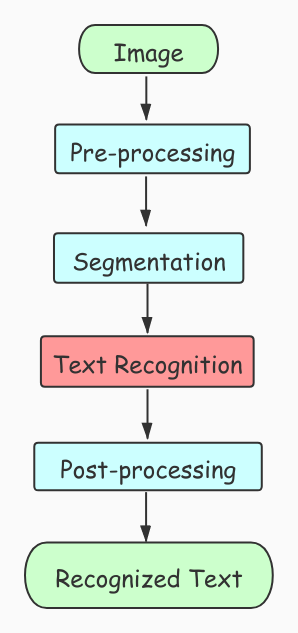
\includegraphics[width=0.25\textwidth]{figure/resources/OCR_system.jpg}
	\caption{光学文本识别系统概览\label{ocr_system_overall}}
\end{figure*}

在过去的三十多年里,学术界已经在 OCR 领域打下了坚实的基础。
这推动了文档图像识别(document image analysis,DIA),多语言,手写体,任意字体 OCR 等就技术的兴起与发展。
所以,当前光学文本识别的研究正在着眼于提高速度和精度的同时,用自然语言的技术去理解和修正文本识别内容的语义正确性。

一套完整的光学文本识别主要包括:

\begin{itemize}
	\item \textbf{预处理}:预处理操作用于提高图片质量及其感兴趣区域。
	\item \textbf{语义结构分割}:虽然语义结构分割可以算是预处理的一部分,不过由于所使用的方法较复杂,且对后面的文本识别有着明显的影响,所以我们将该部分单独作为一个组件。
	\item \textbf{文本识别}:对预处理完的含有文本的图像块进行文本识别,包括字符级识别和字符序列级别。
	\item \textbf{后处理}:虽然目前 OCR 系统(包括端到端的字符序列识别)已经能够到达较高精度,然而它们识别出来的结果依然不可避免的含有一些错误的字符,亦或是缺字多字。后处理就是使用语义模型等复杂模型或字典查询等简单规则对识别结果进行进一步的修正和增强。
\end{itemize}

图\ref{ocr_system_overall}展示了光学文本识别系统的概览,其中文本识别模块是必须的,输入为图像,而其他三个蓝色的模块(预处理,语义结构分割和后处理都是可选的)。

在章节\ref{chap:related_work}介绍研究现状后, 我们将在第\ref{chap:chineseocr}章介绍分析一个典型的案例:ChineseOCR 项目,随后在第\ref{chap:ocr_semantic}章中我们将系统地提出我们的改进思路与工作计划。
最后,我们总结现有文字识别系统并提出展望。

\chapter{研究现状}
\label{chap:related_work}
本章节中我们主要对文本识别系统的框架中每一个组件的研究现状逐一介绍,希望借此为读者提供一个对光学文本识别系统较全面的认识。
首先文本识别系统的框架我们已经在第\ref{chap:introduction}章做了简要介绍,本章节后续内容将围绕该框架展开。
值得一提的是,本章所覆盖的方法只不过是本方向众多论文的冰山一角,难免遗漏了许多有代表性的文章。

\section{预处理}
对于来自扫描仪的图像,一般来说图像质量是比较高的,而许多时候,图像的来源不止扫描仪,还有许多来源于普通的光学相机。
并且,这些来源于光学相机的图像往往有许多噪声和扭曲,甚至有些是在较差的环境下拍摄所得。
为了解决这些图像质量问题以增强图像质量,许多预处理方法被提出。
这些操作一般使用一些比较简单的操作来对所有图像做统一的预处理,包括灰度化,噪声消除,基线识别,偏斜消除。还有一些复杂一点的模型也会被用到,例如文本方向识别。

\begin{figure}[h!]
	\centering
	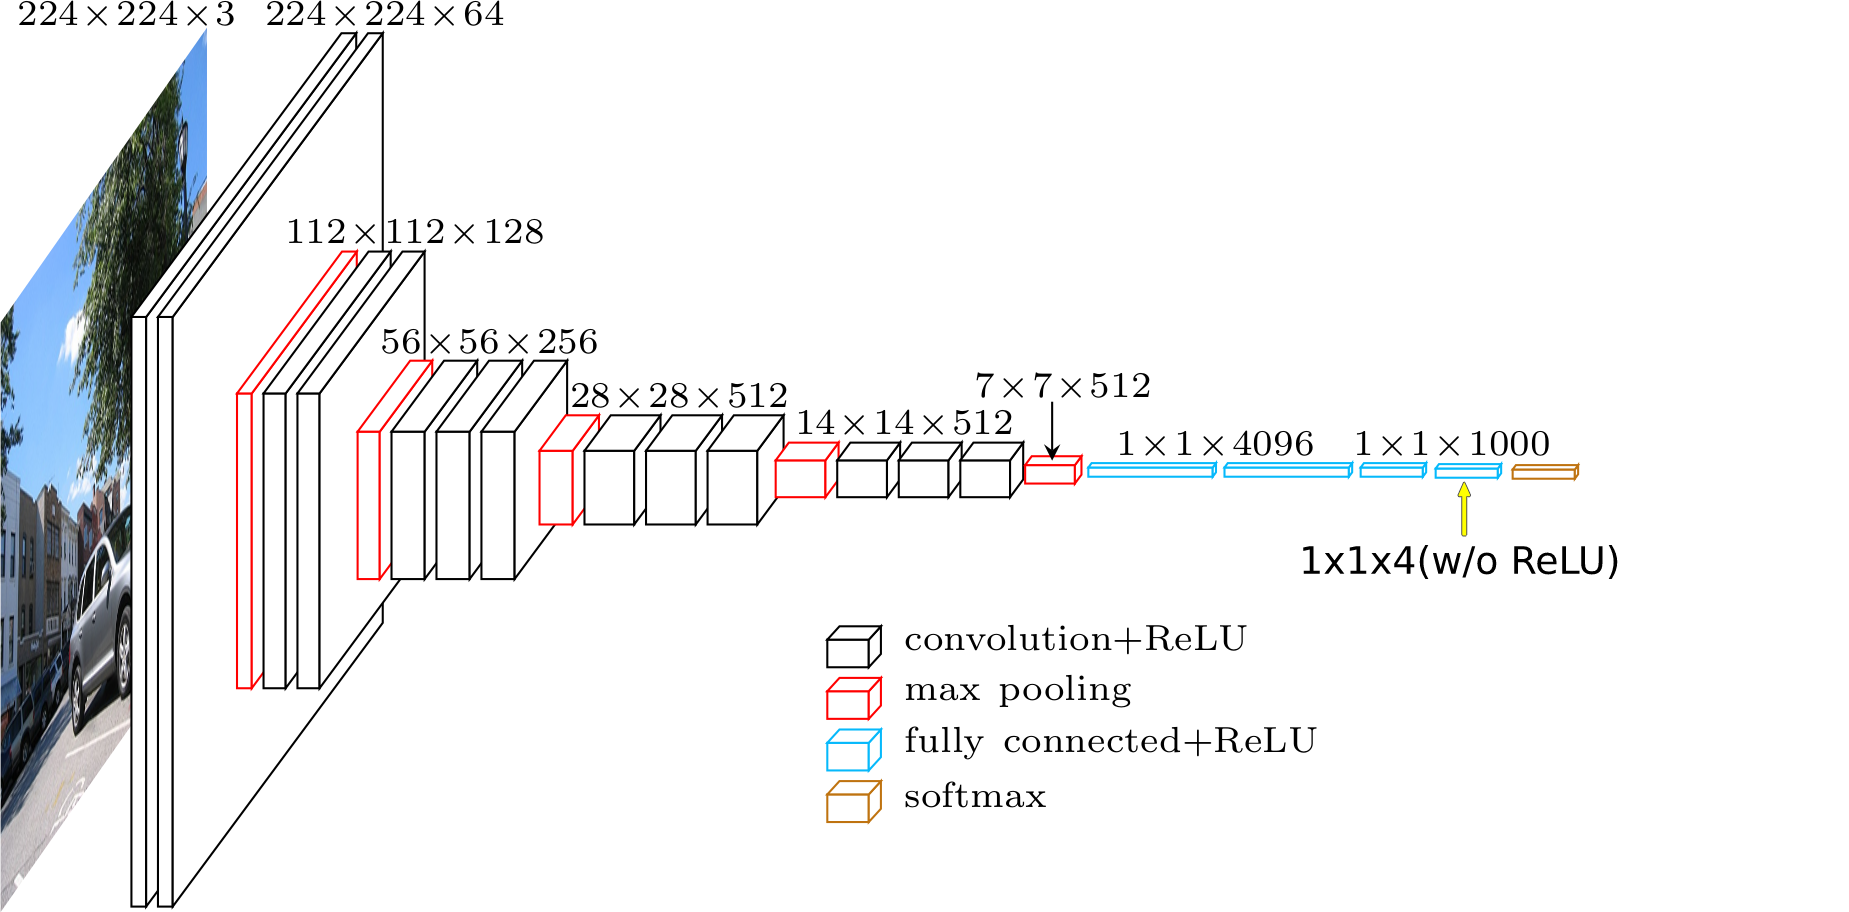
\includegraphics[width=0.75\textwidth]{figure/resources/vgg16_text_angle.png}
	\caption{VGG16 文本方向识别模型\label{vgg16_text_angle}}
\end{figure}

文本识别任务中图像中往往会含有多种方向的文字(0、90、180、270度),所以许多文本识别系统会在预处理的时候进行文字方向识别。
本节介绍一个使用 VGG16\cite{vgg} (项目地址\footnote{Github 仓库:\url{https://github.com/xiaofengShi/CHINESE-OCR/blob/master/angle/predict.py}})进行文本方向的例子。

因为检测结果只有四种文字方向,而原始的 VGG16 是 $1000$ 分类,所以我们需要修改 VGG16 的最后一层全连接层(dense layer)为四分类,经过修改的 VGG16 的整体架构图见图\ref{vgg16_text_angle}。
主要的修改就是在大小为 $1000$ 的全连接层与 softmax 层之间加入一个没有激活单元的大小为 $4$ 的全连接层。

\section{语义结构分割}
传统的 OCR 系统往往以字符为单位进行,也就是每一个图像块有且只有一个字符。而随着深度学习的高速发展,许多学者开始转向使用表达能力更加强的深度学习技术来进行端到端的文本识别(也就是说,直接从整个图像中识别整段文本)。
所以,语义分割的单位也可以分为字符和文本块。

虽然 YOLO 论文中的数据集本身不是用于文本分割的模型,不过我们可以很简单的将 YOLO 用于文本语义分割任务。
按照引用数量和刊物等级,我们介绍一下三种方法:YOLOv3\cite{yolov3},CTPN\cite{CTPN}。
%和MFCNN\cite{MFCNN}。
它们的引用信息和发表情况我们在表\ref{tab:preprocessing_papers}中介绍。

\begin{table}[!hpt]
	\caption[]{语义结构分割有关论文}
	\label{tab:preprocessing_papers}
	\centering
	\begin{tabular}{|c|c|c|c|}
		\hline
		方法 & 引用数\footnotemark & 发表刊物 & 发表时间 \\ [0.5ex] 
		\hline
		YOLO & 7042 & CVPR & 2016 \\
		\hline 
		YOLOv3 & 1752 & - & 2018 \\ 
		\hline
		CTPN & 318 & ECCV & 2016 \\
%		\hline
%		MFCNN & 31 & CVPR & 2017 \\[1ex] 
		\hline
	\end{tabular}
\end{table}
\footnotetext{截止该综述写作时间}

\subsection{YOLO}
YOLO 系列论文由于其高效的速度及可观的识别结果连续几年作为物体识别领域的业界标杆,虽然 YOLO 最初不是用于文本语义结构识别,不过可以很方便地将 YOLO 迁移到文本语义识别领域。

首先我们简要介绍一下 YOLO\cite{YOLO}。
相对于许多组合多个神经网络来进行物体检查论文,YOLO 提出把物体识别当做一个回归问题(regression problem),使用单个网络直接输入图片并输出所有识别出的物体的有界框(bounding boxes)及类别等信息。
虽然 YOLO 对比当时的最新研究(state-of-the-art),精确度低一些,当时 YOLO 的高效及强大的泛化能力是它的亮点。

YOLO 的大致工作流为:首先把图片分成 $S \times S$ 的网格,如果有要识别的物体落在该网格上,则该网格能够反映它识别了该物体。
每个网格预测 $B$ 个有界框及其置信度(因为有多个物体重叠在一个格子里面的情况,所以需要多个格子),这些置信度反映了该框中是否有物体的置信度,置信度定义为 $Pr(Object)*IOU^{\textsf{truth}}_{\textsf{pred}}$,因为作者希望如果框内没有物体,则置信度为 $0$否则作者希望置信度为预测框和实际的 IOU(intersection over union)。
每一个有界框含有五个预测项:$x,y,w,h$ 以及置信度,其中 $x,y$ 表示框中心相对于该网格的距离,$w,h$则表示框的宽度和长度相对于整个图片大小的比值,并且它们都会归一化到 0 到 1 的范围。
每一个网格还需要预测 $C$ 个条件类别概率:$Pr(Class_i|Object)$,这些概率是在该有界框含有物体的条件之下的,值得一提的是 YOLO 没有在同一个网格中为每个有界框预测所有类别的概率。
测试的时候这个条件类别概率乘以每个框的置信度就作为每一个框的类别置信度:$Pr(Class_i|Object)*Pr(Object)*IOU^{\textsf{truth}}_{\textsf{pred}} = Pr(Class_i)*IOU^{\textsf{truth}}_{\textsf{pred}}$。
所以最后我们需要做回归的就是一个大小为$S \times S \times (B * 5 + C)$ 的张量。

\begin{figure}[h!]
	\centering
	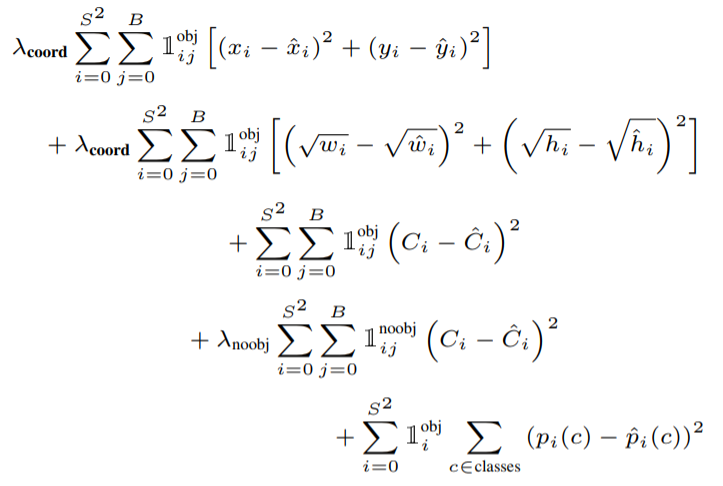
\includegraphics[width=0.5\textwidth]{figure/resources/YOLO_loss.png}
	\caption{YOLO 损失函数\label{YOLO_loss}}
\end{figure}

最后,YOLO 使用基于方差和(sum-squared error)的损失函数见图\ref{YOLO_loss}。
其中,$\lambda_{\text{coord}} = 5, \lambda_{\text{noobj} = 0.5}$ 用来增加有界框的坐标预测的损失值并减少有界框中没有物体时的置信度的损失值。
$\mathbbm{1}_i^{\textsf{obj}}$ 表示如果物体在网格 $i$ 中则为 $1$ 否则为 $0$。
$\mathbbm{1}^{\textsf{obj}}_{ij}$ 表示网格 $i$ 的有界框 $j$ 是有对应的物体(因为不一定所有 $B$ 个框都有物体,很多时候是所有都没有或者只有一个框。
可以很容易看出大部分损失函数只针对有物体的时候。

\subsection{CTPN}
Connectionist Text Proposal Network (CTPN) 直接在卷积层定位文本,这解决了之前许多基于字符检测的自底向上的方法的主要局限。
CTPN 将文本识别问题转化为定位细粒度的文本部件(text proposals)组成的序列的问题,并且作者还开发了一种锚点回归机制(anchor regression mechanism)为每一个文本部件预测垂直位置和是否是文本的置信度,同时在网络内使用循环神经网络来将这些序列文本部件优雅地连接起来。
所以,CTPN 是一个可以处理多语系(multi-lingual)和多尺度(multi-scale)文本的,统一的,端到端的,可训练模型。

因为文本不像一般物体具有封闭的轮廓和明显的中心,文本一般指单词或整段文本,所以整段文本其实是由稀疏的更小的单位(单词,字符,句子)组成,如果直接把文本块当做物体识别,很容易导致识别系统把文本快的部分(例如单词的一部分)当做整个物体。
所以,很容易想到将文本行作为一个细粒度的文本部件组成的序列。
文本部件可以理解为文本行的一小部分,例如,宽度为 $16$ 像素的文本块。
每个文本部件一般包含一个或多个笔画,一个字符的一部分,或者多个字符。
作者认为在固定更难预测的水平位置的情况下,只预测每个文本部件的竖直位置会更加的准确且简单(因为缩小了搜索空间)。

\section{文本识别}
本节中我们主要分析基于深度学习的文本识别模型,其中主要以 Baoguang Shi 等提出的卷积循环神经网络(CRNN)\cite{CRNN}为主要分析对象。
CRNN 是 2017 年发表在 TPAMI 的一篇期刊论文,其引用数目前已有 $583$ 之多,足见起有效性及影响力。

CRNN 是一个集成了特征提取,序列建模和转录(transcription)于一体的端到端的可训练神经网络,并且借助 RNN 的能力,CRNN 很自然地拥有处理任意长度序列的能力,它不需要耦合任何预定义的词库(lexicon)。

\begin{figure}[h!]
	\centering
	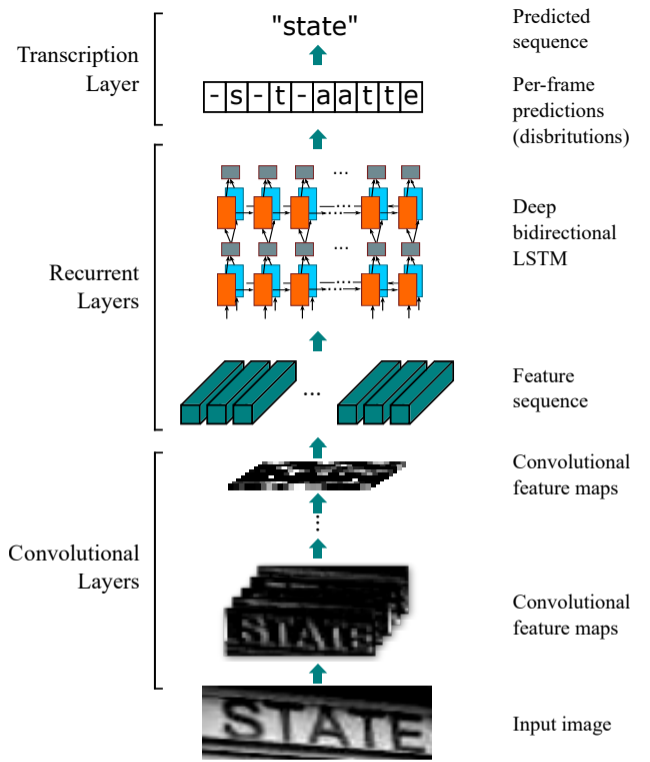
\includegraphics[width=0.5\textwidth]{figure/resources/CRNN_arch.png}
	\caption{CRNN 网络结构\label{CRNN_arch}}
\end{figure}

CRNN 的整体网络结构可见图\ref{CRNN_arch},它输入为固定大小的图像,自底向上主要由三个部分组成:卷积层,循环层和转录层。
卷积层用于从每一张图像中自动提取特征序列,而循环神经网络则用于从特征序列中的每一帧中做出预测,转录层用于将每一帧的 RNN 预测翻译为标签序列。
虽然 CRNN 由多种神经网络组成,但是它可以使用一个损失函数进行联合训练。

特征序列中的每一个特征向量都是从特征图(feature maps)中从左往右按列生成的,也就是说第 $i$ 个特征向量是所有特征图的第 $i$ 列串接而成。
其中每一列的宽度被固定为一个像素。
由于 CNN 的感受野(receptive field)的缘故,特征图的每一列对应原始图片的一个矩形区域,并且从左往右的顺序也是一一对应的。
转录层则是要将 RNN 的逐帧预测输出转化为标签的概率分布。
转录有分为两种:无需词典( Lexicon-free transcription)和基于词典的(Lexicon-based transcription),词典就是一组固定的标签序列,例如一个拼写检查词典。
无需词典模式就是说预测结果不需要借助任何词典,而词典模式就是寻找概率最大的标签序列。
CRNN 使用 CTC (Connectionist Temporal Classification ,连通时域分类)层作为条件概率。

\begin{figure}[h!]
	\centering
	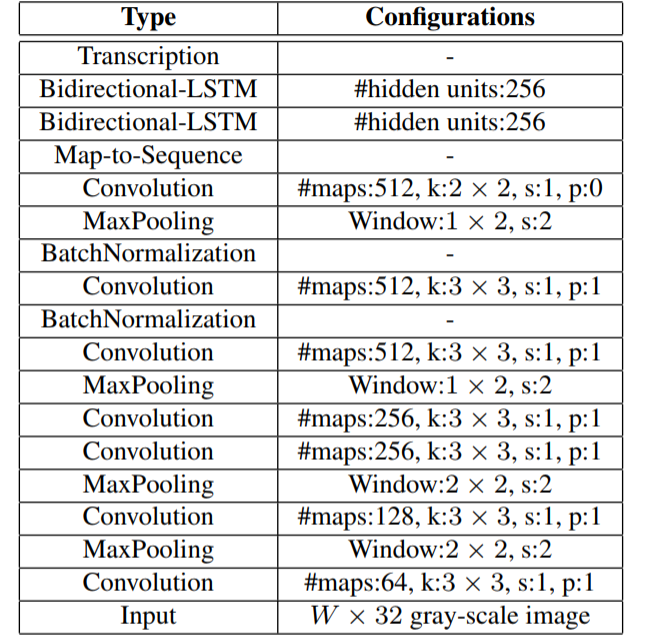
\includegraphics[width=0.6\textwidth]{figure/resources/CRNN_conf.png}
	\caption{CRNN 网络配置\label{CRNN_conf}}
\end{figure}

CRNN 网络的具体配置可见图\ref{CRNN_conf}。

\section{基于语义分析的后处理}
虽然现有的 OCR 系统已经有很高的精确度和较强的范化能力了,但是仍然不可避免地含有个别错误,比如错字,缺字多字。
同时,NLP 领域已经发展地比较成熟了,我们可以使用 NLP 的技术来对 OCR系统识别出的结果已经后处理,精细化和处理少数错误。
但是相对于英语法语这样的字母语言,中文不仅词汇量大,而且由于中文书写的复杂性,中文拼写错误纠正更加难以解决。
例如”今天的天气很好“很容易被错误识别为”令天的天气很好“。
再加之中文没有明显的分词界限,不同的分词也许代表完全不一样的语义,中文文字识别的后处理因此变得更加棘手。
拼写检查大致分为基于规则的和基于统计的方法,显然基于规则的方法会更有局限性,而统计方法具有很好的鲁棒性。
所以综上所述,造成中文文本系统的后处理任务的困难之处主要在于:
\begin{enumerate}
	\item 汉字的词汇量大,且含有大量相似字,同义字,再加之中文书写和语法的复杂性。
	\item 中文没有明显的分词界限,不同的分词也许代表完全不一样的语义。
	\item 文本在不同工作环境下有明显特征(例如发票),但是缺少拼写检查有关的大型数据集,大部分数据只有图片和文本的对应关系。
\end{enumerate}

本章中,我们主要简要介绍一个基于机器学习的方法,简称为基于SMT(Statistical Machine Translation)的方法\cite{post_SMT}和基于LSTM的方法\cite{post_LSTM}。
% 这些方法的发表情况见表\ref{tab:postprocessing}。
基于LSTM的方法\cite{post_LSTM}我们将在关键技术介绍部分作展示。

\subsection{基于 SMT 的方法}
该论文基于短语统计机器翻译(phrasal statistical machine translation)框架来进行中文拼写错误检测和修正,该方法结合了基于规则的方法和基于统计的方法,使用统计模型来解决基于规则的方法忽视上下文的问题。
大致的思路主要分为以下三个部分:
\begin{enumerate}
	\item 中文句子被分段为词。
	\item 检测模块用于检测和标记可能有拼写错误的词。
	\item 在错误修正阶段,使用 SMT 模型来将含有拼写错误的句子转化为正确的。
\end{enumerate}

使用分词来减小搜索空间和错误率,不过中文分词常常会出现过分词(over-segmented )现象,SMT 模型则可用于解决该问题。
例如“除了要有超世之才,也要有堅定的意志”可能被过分词为:“除了/要/有/超世/之/才/,/也/要/有/堅定/的/意
志”。
扩充词典也是一种解决方案。
因为拼写错误往往导致一串单字出现在分词结果中,所以所有由单字导出的 $n$-grams将考虑作为候选错误词(candidates)。
该方法有个潜在的局限性就是,如果词组不在词典里面,则它们会被视作拼写错误。

找出拼写错误的列表后,SMT 尝试将句子翻译为正确的形式。
当给定一个拼写错误的词,首先通过将字符替换为相似的字,一次替换一个,来生成所有的正确假设。
例如对于“氣份”一词,部分正确假设为:汽份,泣份,
器份, 契份,
企份, 憩份,
氣分, 氣忿,
氣憤, 氣糞,
氣奮, 氣氛。
这些翻译假设将使用词典来验证(修剪)。
翻译概率定义为:
\begin{equation}
tp = \log_{10} \left(\frac{freq(trans)}{freq(trans) - freq(condi)}\right)*\gamma
\end{equation}

解码器用于单调的(也就是不改变原来语序)翻译语法错误,翻译模型使用GIZA++,语言模型使用 SRILM。

\begin{table}[!hpt]
	\caption[]{SMT 翻译样例}
	\label{tab:preprocessing_papers}
	\centering
	\begin{tabular}{|c|c|c|c|}
		\hline
		翻译 & 频率 & 语言模型概率 & tp \\ [0.5ex] 
		\hline
		氣憤 & 48 & -4.96 & -1.20 \\
		\hline
		氣氛 & 473 & -3.22 & -1.11 \\[1ex] 
		\hline
	\end{tabular}
\end{table}

\chapter{案例分析: ChineseOCR}
\label{chap:chineseocr}

ChineseOCR 是结合了近几年最新论文成果的综合项目,其主要借鉴的模型有:YOLOv3(用作单个字符识别),AngleDetect(VGG),CTPN(文本线检测模型)及CRNN。
数据集采用 $\sim 500w$ 条数据,其中 $20\%$ 为真实数据,$80\%$ 为合成数据,并且因为使用了一部分私有数据,所以数据集并不是公开的。
ChieseOCR 可以视作是一个多阶段(multi-stage)文本识别模型,因为每一个部分都是单独训练的。

\begin{figure}[h!]
	\centering
	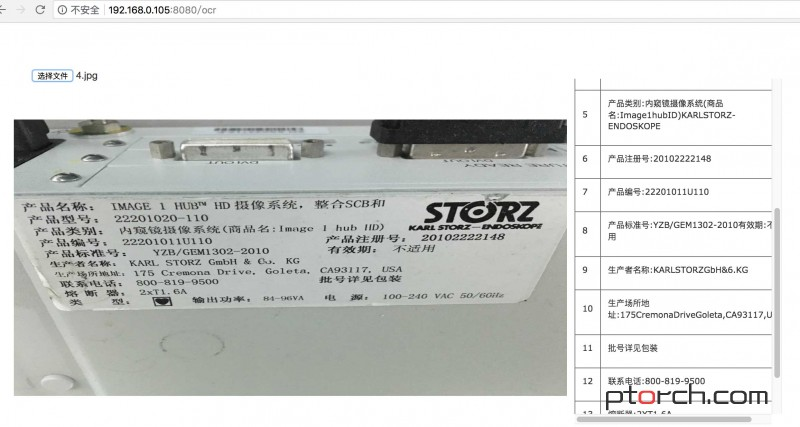
\includegraphics[width=0.7\textwidth]{figure/resources/chineseocr_ex1.jpg}
	\caption{ChineseOCR 应用举例\label{chineseocr_ex1}}
\end{figure}

\begin{figure}[h!]
	\centering
	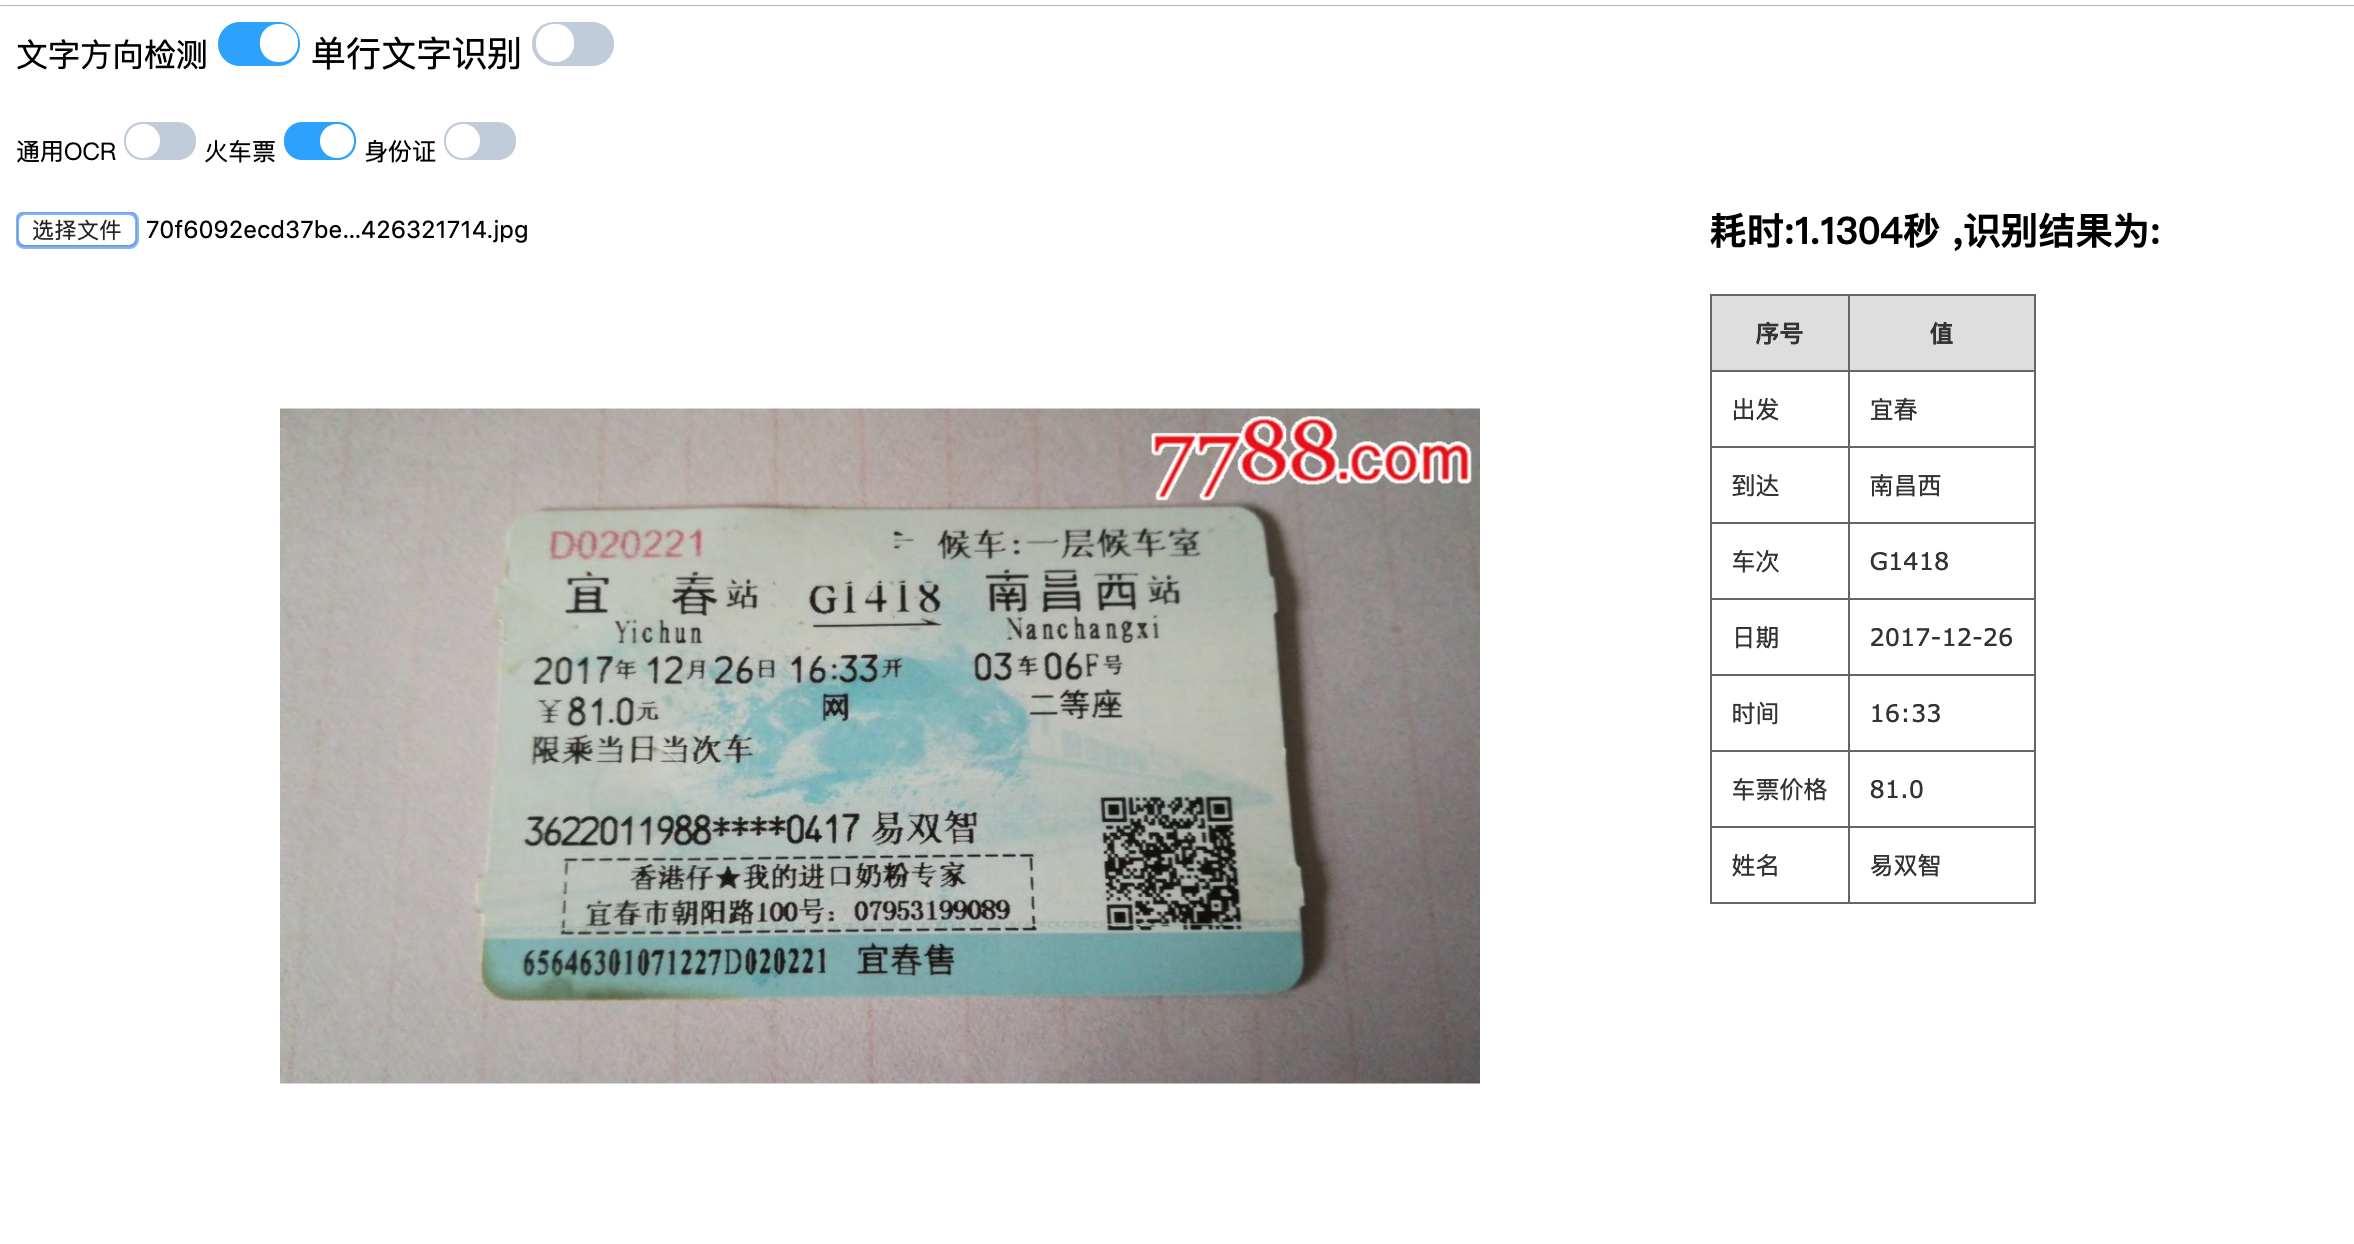
\includegraphics[width=0.7\textwidth]{figure/resources/chineseocr_struct.png}
	\caption{ChineseOCR 结构化识别举例\label{chineseocr_structure}}
\end{figure}

一些 ChineseOCR 的应用场景的例子可见图\ref{chineseocr_ex1}和图\ref{chineseocr_structure}。

\section{系统架构}

\begin{figure}[h!]
	\centering
	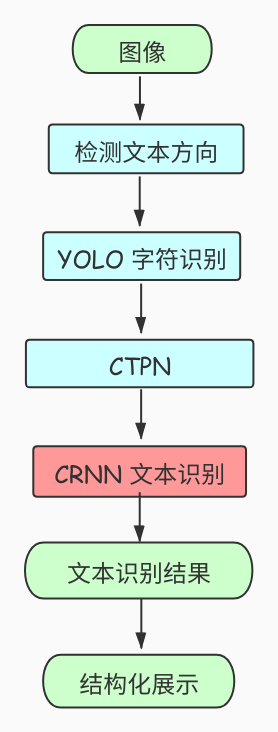
\includegraphics[width=0.25\textwidth]{figure/resources/chineseocr.jpg}
	\caption{ChineseOCR 工作流\label{chineseocr_structure}}
\end{figure}

ChineseOCR 的工作流如图\ref{chineseocr_structure}所示。

\section{优劣之处}
ChineseOCR 因为是目前较新方法组合而成,加之数据集规模较大,所以测试结果很不错。
并且 ChineseOCR 有一个亮点就是它将最后的识别结果再做了一些结构化处理,比如针对火车票和身份证。
不过目前为止,ChineseOCR 主要有以下几点不足:
\begin{itemize}
	\item 结构化处理目前只有身份证和火车票,仍然还有其他大量的类似任务,可以考虑将这类结构化处理任务配置为统一格式,只需要用户自行添加一个格式描述文件即可增加支持的任务。
	\item 缺乏后处理,目前 ChineseOCR 完全没有后处理。后处理包括简单的词典规则匹配,或复杂的基于语言模型或注意你机制下的LSTM模型都是很有意义的改进方向。同时可以考虑使用机器翻译的复杂模型(例如 BERT)迁移到后处理任务来。
	\item 数据集不公开,无法复现,需要自己重新收集大规模数据集。
\end{itemize}

\chapter{课题研究内容}
本章节我们主要介绍本科研研究的内容,我们的目标是实现一个完整的面向语义分析的文本识别系统,其架构图在图\ref{system_overall} 中展示。

\begin{figure}[h!]
	\centering
	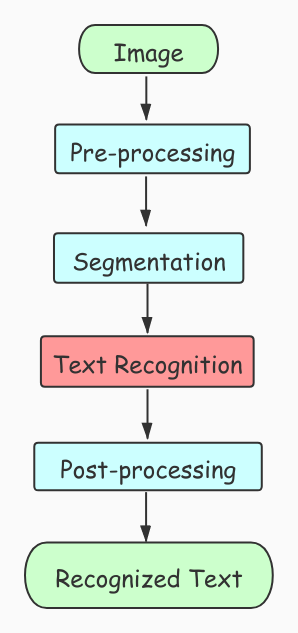
\includegraphics[width=0.25\textwidth]{figure/resources/OCR_system.jpg}
	\caption{面向语义分析的文本识别系统架构图\label{system_overall}}
\end{figure}

详细的任务包括:
\begin{itemize}
	\item 实现一个完整的面向语义分析的文本识别系统。
	\item 使用语义模型、语言模型对完善文本识别系统的后处理组件,基于语义分析对文本结果进行修正,参考第\ref{sec:lstm_based_postprocessing}章中的论文。
	\item 我们将考虑使用预训练的机器翻译模型(例如 BERT)迁移学习到本任务中去,并且将论文中的注意力机制和 RNN 更改为自注意力机制和 Transformer 架构,以解决 LSTM 获取长距离依赖信息以及获取(平移不变的)局部信息能力较弱的问题。
	\item 针对特定任务优化数据集,比如在税务发票识别任务时我们使用税务发表的数据集(并且经过数据增强)对我们的预训练模型进行细粒度调校(fine-tune)。
	\item 增加更加通用的结构化处理机制,将这类结构化处理任务配置为统一格式,只需要用户自行添加一个格式描述文件即可增加支持的任务。
\end{itemize}


\chapter{技术路线}
\label{chap:ocr_semantic}

\section{数据集与数据增强}
基于深度学习的模型往往需要大量数据以得到具有足够的范化能力的模型,目前公开的文本识别数据集主要有以下几个:
\begin{enumerate}
	\item \textbf{Chinese Text in the Wild(CTW)\cite{yuan2019ctw}}: 该数据集包含32285张图像,1018402个中文字符(来自于腾讯街景), 包含平面文本,凸起文本,城市文本,农村文本,低亮度文本,远处文本,部分遮挡文本。图像大小2048*2048,数据集大小为31GB。以(8:1:1)的比例将数据集分为训练集(25887张图像,812872个汉字),测试集(3269张图像,103519个汉字),验证集(3129张图像,103519个汉字)。
	\item \textbf{Reading Chinese Text in the Wild(RCTW-17)\cite{ICDAR2017}}:该数据集包含12263张图像,训练集8034张,测试集4229张,共11.4GB。大部分图像由手机相机拍摄,含有少量的屏幕截图,图像中包含中文文本与少量英文文本。图像分辨率大小不等。
	% \footnote{\url{https://tianchi.aliyun.com/competition/information.htm?raceId=231651\&\_is\_login\_redirect=true\&accounttraceid=595a06c3-7530-4b8a-ad3d-40165e22dbfe}
	\item \textbf{ICPR MWI 2018 挑战赛}: 大赛提供20000张图像作为数据集,其中50\%作为训练集,50\%作为测试集。主要由合成图像,产品描述,网络广告构成。该数据集数据量充分,中英文混合,涵盖数十种字体,字体大小不一,多种版式,背景复杂。文件大小为2GB。
	%\item \textbf{Total-Text}\footnote{\url{http://www.cs-chan.com/source/ICDAR2017/totaltext.zip}}: 该数据集共1555张图像,11459文本行,包含水平文本,倾斜文本,弯曲文本。文件大小441MB。大部分为英文文本,少量中文文本。训练集:1255张 测试集:300
	% \item \textbf{Google FSNS(谷歌街景文本数据集)}\footnote{http://rrc.cvc.uab.es/?ch=6\&com=downloads}: 该数据集是从谷歌法国街景图片上获得的一百多万张街道名字标志,每一张包含同一街道标志牌的不同视角,图像大小为600*150,训练集1044868张,验证集16150张,测试集20404张。
	% \item \textbf{COCO-TEXT}\footnote{https://vision.cornell.edu/se3/coco-text-2/}: 该数据集,包括63686幅图像,173589个文本实例,包括手写版和打印版,清晰版和非清晰版。文件大小12.58GB,训练集:43686张,测试集:10000张,验证集:10000张
\end{enumerate}

% \footnote{\url{http://www.robots.ox.ac.uk/~ankush/textloc.pdf}}
% \footnote{\url{https://github.com/Aurora11111/TextRecognitionDataGenerator}}
此外,还有一些合成数据集及合成算法:Synthetic Data for Text Localisation 和 Text Recognition Data Generator。
% \footnote{\url{https://github.com/microsoft/VoTT}}
当然也可以自己标注,标注软件可以使用微软 VoTT。
数据增强即采用各种图形学手段(形变,缩放,饱和度和曝光等)扩充数据集,避免模型训练过程中出现过拟合情况。

\section{面向语义分析的文本识别系统}
我们将要研究实现的面向语义分析的文本识别系统主要包括以下几个部件,我们将简要介绍其技术:

\begin{itemize}
	\item \textbf{预处理}:使用 OpenCV 等成熟的图像处理函数库进行预处理操作,用于提高图片质量及其感兴趣区域,使用 VGG 用作文本方向识别。
	\item \textbf{语义结构分割}:使用 YOLO 或 CTPN 用作语义分割。
	\item \textbf{文本识别}:使用 CRNN 对预处理完的含有文本的图像块进行字符序列级别文本识别,或者提出一个新的神经网络架构,整个语义结构分割和文本识别这两个组件为一个组件。
	\item \textbf{后处理}:使用基于注意力机制的 LSTM 架构来进行基于语义的字符级修正,同时将考虑使用自注意力机制和预训练语言模型(例如 BERT 机器翻译模型)迁移到后处理任务。
\end{itemize}

\chapter{关键技术介绍}
我们的课题主要将基于以下核心技术进行改进与扩展。

\section{基于注意力机制和 LSTM 的方法}
\label{sec:lstm_based_postprocessing}
该论文提出使用基于注意力机制的深度学习网络结合迷糊集(confusion sets)来进行字符级中文拼写错误的检测与修正。
模型首先使用 LSTM 来建模中文词嵌入(Chinese character embedding)的上下文,然后使用注意力机制从迷惑集中为候选词打分,选择分数最高的作为预测项。
同时,该论文提供了一个数据集\footnote{\url{https://github.com/ccit-proofread}},并提供了了一种获取(前序文本,后序文本,候选词,目标)四元组的作为数据集的方法。

本方法的主要贡献有:
\begin{enumerate}
	\item 通过在字符级(char-level)处理来避免分词产生的误差。
	\item 收集字符级迷惑集(character-level confusion sets)作为先验知识来减少推荐的正确候选词的数量。
	\item 使用编码器来提取更加全局的信息来减少局部错误的影响,使用置信度阈值来使得模型更好地适应不同的错误率的文本。
\end{enumerate}

一般的注意力机制被定义为:
\begin{equation}
\begin{gathered}
r(h_t, h_s) = h_t^T W_a h_s \\
a_t(s) = softmax(r(h_t, h_s)) \\
c_t = \sum_s a_s(s) h_s
\end{gathered}
\end{equation}
其中$W_a \in \mathbb{R}^{\lVert h_t^T \rVert \times \lVert h_s \rVert}$, $h_s$ 和 $h_t$ 分别为源和目的隐藏状态,$r(\cdot, \cdot)$ 为关系分数。

论文基于注意力机制,提出两种基于注意力机制的模型。

\chapter{要解决的技术问题}
基于 ChineseOCR 以下几个不足之处:
\begin{itemize}
	\item 结构化处理目前只有身份证和火车票,仍然还有其他大量的类似任务,可以考虑将这类结构化处理任务配置为统一格式,只需要用户自行添加一个格式描述文件即可增加支持的任务。
	\item 缺乏后处理,目前 ChineseOCR 完全没有后处理。后处理包括简单的词典规则匹配,或复杂的基于语言模型或注意你机制下的LSTM模型都是很有意义的改进方向。同时可以考虑使用机器翻译的复杂模型(例如 BERT)迁移到后处理任务来。
	\item 数据集不公开,无法复现,需要自己重新收集大规模数据集。
\end{itemize}


\begin{table}[!hpt]
	\caption[]{工作计划\label{tab:work_plan}}
	\centering
	\begin{tabular}{|c|c|c|}
		\hline
		项目 & 时间安排 & 备注 \\ [0.5ex] 
		\hline
		阅读文献,确定思路 & 2019/10/09$\Rightarrow$2019/11/27 & 已完成  \\ 
		\hline
		准备数据集,实现代码原型 & 2020/01/01$\Rightarrow$2020/03/01 & 同时继续阅读文献  \\ 
		\hline
		完善系统,提高性能 & 2020/03/02$\Rightarrow$2020/04/01 & 增加功能  \\
		\hline
		撰写论文 & 2020/04/02$\Rightarrow$2020/05/01 & 完善功能演示 \\[1ex] 
		\hline
	\end{tabular}
\end{table}

这些不足点导致我们对 ChineseCOR 基本没有扩展能力,并且不符合我们语义分析的目的以及指定任务的文本识别的需求,我们提出以下改进措施:
\begin{itemize}
	\item 使用语义模型、语言模型对完善文本识别系统的后处理组件,基于语义分析对文本结果进行修正,参考第\ref{sec:lstm_based_postprocessing}章中的论文。并且,我们将考虑使用预训练的机器翻译模型(例如 BERT)迁移学习到本任务中去,并且将论文中的注意力机制和 RNN 更改为自注意力机制和 Transformer 架构,以解决 LSTM 获取长距离依赖信息以及获取(平移不变的)局部信息能力较弱的问题。
	\item 针对特定任务优化数据集,比如在税务发票识别任务时我们使用税务发表的数据集(并且经过数据增强)对我们的预训练模型进行细粒度调校(fine-tune)。
	\item 增加更加通用的结构化处理机制,将这类结构化处理任务配置为统一格式,只需要用户自行添加一个格式描述文件即可增加支持的任务。
\end{itemize}

\chapter{日程安排}
详细的工作计划我们将在表\ref{tab:work_plan}中详细阐述。

\chapter{总结与展望}
\label{chap:conclusions}  
本文较为系统全面的分析了目前文本识别系统的一般框架及其最新技术,不足之处在于文本识别系统和其他几个部件还需要更多的有代表性的文章以给老师们一个更加全面的描述。
文本识别系统依然存在着大量的改进空间,不管是在 CRNN 这样的单阶段(single-stage)系统上加入更加复杂的 NLP 领域深度学习有关技术(例如,BERT 预训练模型的迁移学习,或者将使用的注意力机制更换为自注意力机制),还是在多阶段(multi-stage)系统中加入更多的基于语义分析的后处理模型,都是值得研究探讨的方向。
希望能够借助此文给老师们清楚地描述本课题的工作方向及计划,初次接触该方向,如有不足之处,还烦请指证!

% \end{summary}